%\iffalse
\let\negmedspace\undefined
\let\negthickspace\undefined

\documentclass[journal,12pt,onecolumn]{IEEEtran}

\usepackage{cite}
\usepackage{amsmath,amssymb,amsfonts,amsthm}
\usepackage{graphicx}
\usepackage{textcomp}
\usepackage{xcolor}
\usepackage{txfonts}
\usepackage{listings}
\usepackage{enumitem}
\usepackage{mathtools}
\usepackage{gensymb}
\usepackage[breaklinks=true]{hyperref}
\usepackage{tkz-euclide}
\usepackage{listings}
\usepackage{float}
\usepackage{subcaption}
\usepackage{listings}

\newtheorem{theorem}{Theorem}[section]
\newtheorem{problem}{Problem}
\newtheorem{proposition}{Proposition}[section]
\newtheorem{lemma}{Lemma}[section]
\newtheorem{corollary}[theorem]{Corollary}
\newtheorem{example}{Example}[section]
\newtheorem{definition}[problem]{Definition}
\newcommand{\BEQA}{\begin{eqnarray}}
\newcommand{\EEQA}{\end{eqnarray}}
\newcommand{\define}{\stackrel{\triangle}{=}}
\theoremstyle{remark}
\newtheorem{rem}{Remark}
\lstset{
    language=Matlab, % Set the programming language to MATLAB
    caption=Example MATLAB code, % Set the caption
    label=lst:matlab-example, % Set the label for referencing
    basicstyle=\ttfamily, % Set the basic style (typewriter font)
    breaklines=true, % Enable automatic line breaking
    numbers=left, % Show line numbers on the left
    frame=single, % Add a frame around the code
    keywordstyle=\color{blue}, % Set the style for keywords
    commentstyle=\color{green!60!black}, % Set the style for comments
    stringstyle=\color{red}, % Set the style for strings
    morekeywords={matlab2tikz}, % Add additional MATLAB keywords
}

\begin{document}

\providecommand{\pr}[1]{\ensuremath{\Pr\left(#1\right)}}
\providecommand{\prt}[2]{\ensuremath{p_{#1}^{\left(#2\right)} }}
\providecommand{\qfunc}[1]{\ensuremath{Q\left(#1\right)}}
\providecommand{\sbrak}[1]{\ensuremath{{}\left[#1\right]}}
\providecommand{\lsbrak}[1]{\ensuremath{{}\left[#1\right.}}
\providecommand{\rsbrak}[1]{\ensuremath{{}\left.#1\right]}}
\providecommand{\brak}[1]{\ensuremath{\left(#1\right)}}
\providecommand{\lbrak}[1]{\ensuremath{\left(#1\right.}}
\providecommand{\rbrak}[1]{\ensuremath{\left.#1\right)}}
\providecommand{\cbrak}[1]{\ensuremath{\left\{#1\right\}}}
\providecommand{\lcbrak}[1]{\ensuremath{\left\{#1\right.}}
\providecommand{\rcbrak}[1]{\ensuremath{\left.#1\right\}}}
\newcommand{\sgn}{\mathop{\mathrm{sgn}}}
\providecommand{\abs}[1]{\left\vert#1\right\vert}
\providecommand{\res}[1]{\Res\displaylimits_{#1}} 
\providecommand{\norm}[1]{\left\lVert#1\right\rVert}
\providecommand{\mtx}[1]{\mathbf{#1}}
\providecommand{\mean}[1]{E\left[ #1 \right]}
\providecommand{\cond}[2]{#1\middle|#2}
\providecommand{\fourier}{\overset{\mathcal{F}}{ \rightleftharpoons}}
\newenvironment{amatrix}[1]{%
  \left(\begin{array}{@{}*{#1}{c}|c@{}}
}{%
  \end{array}\right)
}
\newcommand{\solution}{\noindent \textbf{Solution: }}
\newcommand{\cosec}{\,\text{cosec}\,}
\providecommand{\dec}[2]{\ensuremath{\overset{#1}{\underset{#2}{\gtrless}}}}
\newcommand{\myvec}[1]{\ensuremath{\begin{pmatrix}#1\end{pmatrix}}}
\newcommand{\mydet}[1]{\ensuremath{\begin{vmatrix}#1\end{vmatrix}}}
\newcommand{\myaugvec}[2]{\ensuremath{\begin{amatrix}{#1}#2\end{amatrix}}}
\providecommand{\rank}{\text{rank}}
\providecommand{\pr}[1]{\ensuremath{\Pr\left(#1\right)}}
\providecommand{\qfunc}[1]{\ensuremath{Q\left(#1\right)}}
	\newcommand*{\permcomb}[4][0mu]{{{}^{#3}\mkern#1#2_{#4}}}
\newcommand*{\perm}[1][-3mu]{\permcomb[#1]{P}}
\newcommand*{\comb}[1][-1mu]{\permcomb[#1]{C}}
\providecommand{\qfunc}[1]{\ensuremath{Q\left(#1\right)}}
\providecommand{\gauss}[2]{\mathcal{N}\ensuremath{\left(#1,#2\right)}}
\providecommand{\diff}[2]{\ensuremath{\frac{d{#1}}{d{#2}}}}
\providecommand{\myceil}[1]{\left \lceil #1 \right \rceil }
\newcommand\figref{Fig.~\ref}
\newcommand\tabref{Table~\ref}
\newcommand{\sinc}{\,\text{sinc}\,}
\newcommand{\rect}{\,\text{rect}\,}
\let\vec\mathbf
\bibliographystyle{IEEEtran}
\bigskip

\begin{center}
EM ASSIGNMENT \\
BY ADITI DURE(ee23BTech11016) and E MOHANA(ee23BTech11018)
\end{center}

\pagebreak
\pagebreak

Q2: Consider the charge configuration :-

\begin{figure}[h]
  \centering
  \begin{subfigure}{0.3\textwidth}
    \centering
    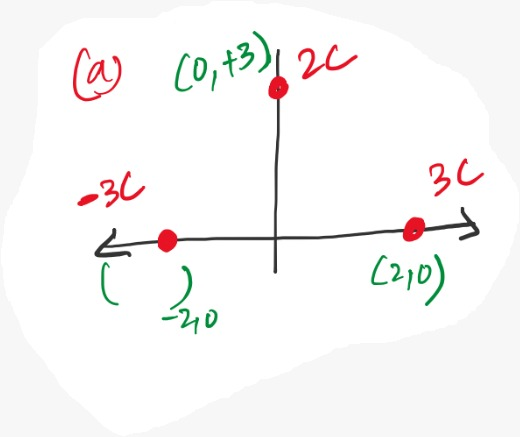
\includegraphics[width=\linewidth]{q1.jpeg}
  \end{subfigure}
  \begin{subfigure}{0.3\textwidth}
    \centering
    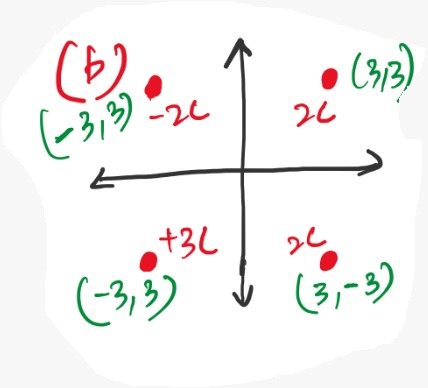
\includegraphics[width=\linewidth]{q2.jpeg}
  \end{subfigure}
  \begin{subfigure}{0.3\textwidth}
    \centering
    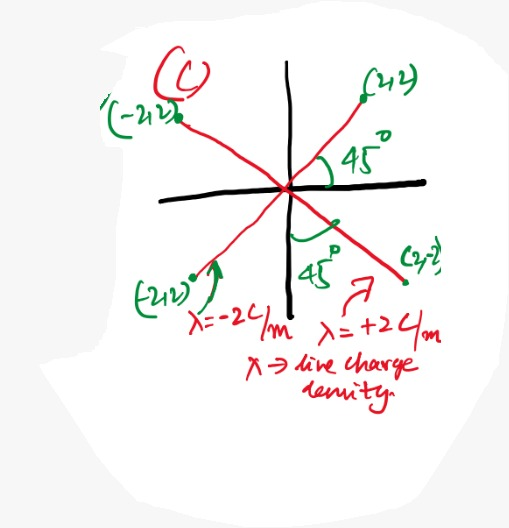
\includegraphics[width=\linewidth]{q3.jpeg}
  \end{subfigure}
\end{figure}

2.1) PLot for all charge configuration for ($\pm$ 6, $\pm$ 6) \\
a) $\vec{E}$ \\
\solution
a) source code:
\begin{lstlisting}
%constants
k = 9 * 10^9;

%charges
q1 = 2;
q2 = -3;
q3 = 3;

%creating grid
[x, y] = meshgrid(-6:0.5:6, -6:0.5:6);

%value of x and y component of Electric Field
Ex = k * q1 * x ./ (x.^2 + (y - 3).^2).^(3/2) + ...
     k * q2 * (x + 2) ./ ((x + 2).^2 + y.^2).^(3/2) + ...
     k * q3 * (x - 2) ./ ((x - 2).^2 + y.^2).^(3/2);

Ey = k * q1 * (y - 3) ./ (x.^2 + (y - 3).^2).^(3/2) + ...
     k * q2 * y ./ ((x + 2).^2 + y.^2).^(3/2) + ...
     k * q3 * y ./ ((x - 2).^2 + y.^2).^(3/2);

%plotting
figure;
quiver(x, y, Ex, Ey, 'Color', 'r');
xlabel('x');
ylabel('y');
title('Electric Field');
\end{lstlisting}



b) V \\
c) U (Electrostatic Energy) \\

\end{document}
